\documentclass[hyperref={pdfpagelabels=true}]{beamer}

\usepackage{lmodern}
\usepackage{hyperref}
\usepackage{caption}
 
\title{Predictive Analysis of Road Incidences}   
\subtitle{Exploratory Lines}
\author{BDigital} 
\date{\today} 
\titlegraphic{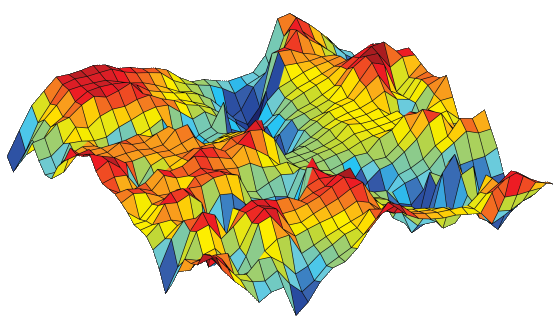
\includegraphics[width=.45\textwidth,height=.35\textheight]{som.png}}
 
\usepackage{beamerthemeshadow}
%\usepackage{beamerthemesplit}
\usepackage{listings}

\newcommand{\soooo}{H$_2$SO$_4$}

%fdl stuff
\usepackage{hyperref}
\hypersetup{colorlinks, 
           citecolor=black,
           filecolor=black,
           linkcolor=black,
           urlcolor=black,
           bookmarksopen=true,
           pdftex}

\hfuzz = .6pt % avoid black boxes


\begin{document}

\captionsetup{font=scriptsize,labelfont=scriptsize}

\setbeamertemplate{footline}[page number]
\setbeamertemplate{navigation symbols}{}
\begin{frame}
\titlepage
\end{frame} 
 
\begin{frame}
\frametitle{Introduction}
\begin{overprint}
\begin{itemize}
\item Despite significant improvements in vehicle technology and road engineering over the last 40 years, on a world-wide scale 
road accidents are still one of the main accidental causes of death and injury (WHO, 2004).\\
%The assessment of the occurrence of road accidents and the management of infrastructure to deal with this risk are therefore research areas of considerable interest. 
\item In a study regarding the relation between extreme weather events (e.g.: flash floods) and road accidents it was found that motorists account for 84 \% of the totality of the
victims [cite].
%Identification of factors that affect the occurrence of road accidents has attracted the attention of many researchers in the field of traffic
%safety.\\%Recognizing such elements may help not only to reduce the number of deaths in traffic crashes, but also the number of accidents with severe injuries [cite].\\ 
\item The assessment of the occurrence of road accidents has therefore attracted the attention of many researchers.
\end{itemize}
\end{overprint}
\end{frame}
\begin{frame}
\frametitle{Introduction (cont.)}
\begin{figure}
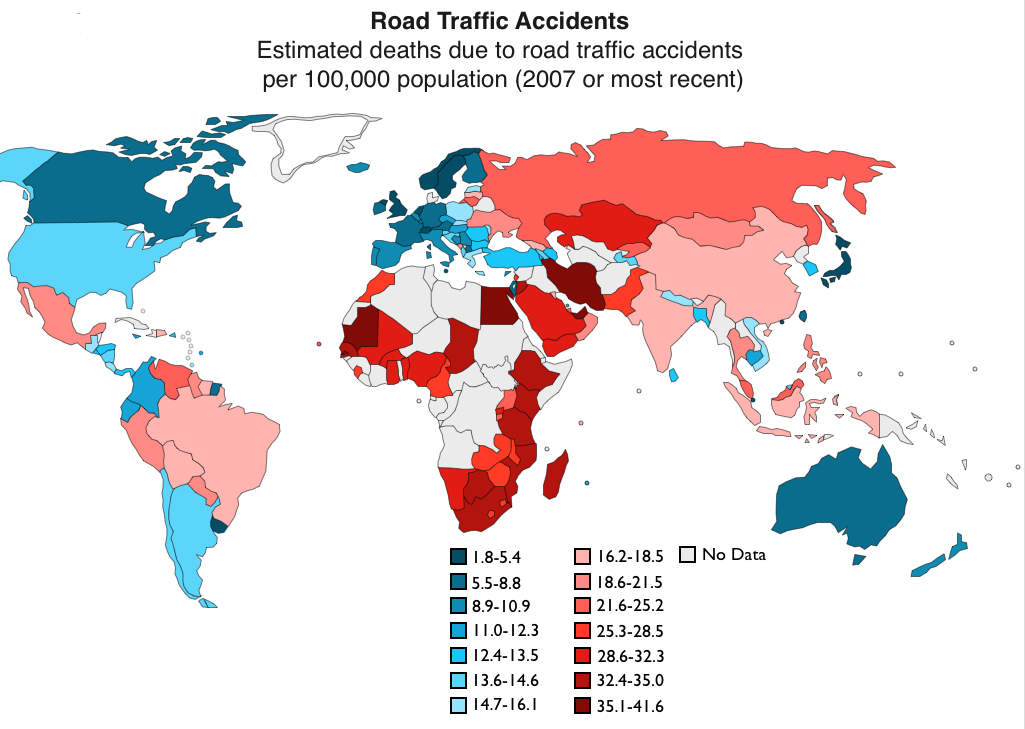
\includegraphics[scale=0.25]{world_accidents.png}
\end{figure}
\tiny{source: {\url http://www.geocurrents.info}}
\end{frame}

\begin{frame}
\frametitle{Research Question}
\textbf{ What do we want to predict?}\\
Ocurrence (0,1) and location (x,y) of incidents, as a function (pairwise or multivariant) of other variables;
\small{
\begin{itemize}
\item time of the day;
\item weekday;
\item traffic density;
\item weather (rainfall, snowfall, visibility, winds, etc);
\item traffic control devices (e.g.: traffic lights, stop signal, etc);
\item roadway geometries (e.g.: steepness, intersection, degree of curvature, etc) 
%\footnote{\tiny{Factors reflecting basic road geometry and traffic volumes have been demonstrated to have a 95\% significance level[cite]}}
;
\item roadway conditions (road surface, obstacles);
%\item driver behavior
\item vehicle type;
\item human conditions (characteristics of the driver, fatigue, alcohol);
\item involvement of pedestrians;
\end{itemize}
}
Some of these variables are continuous in space and most of them change over time.\\
\end{frame}

\begin{frame}
\frametitle{Modelling Approaches: Classical Statistics}
\begin{itemize}
\item<1-> The most common approach applied in early works is to model the interaction between each dependent variable and accident frequencies by means of conventional (multiple) linear
regression models[cite]; these \textbf{do not take in account covariance between response variables}. 
\item<2-> Most of these models use a Normal or Poisson distribution that is not well-suited to the scarce nature of accident data. Accident data is often characterized by small observed mean values and a large number of zero counts leading to the well discussed phenomenon of \textbf{over-dispersion}: the presence of greater variability (statistical dispersion) in a data set than would be expected based on a given simple statistical model.
\item<3-> None of these models addresses explicitly the question of \textbf{spatial autocorrelation}: the value of samples taken close to each other are more likely to have similar magnitude than by chance alone.
\end{itemize}
\end{frame}

\begin{frame}
\frametitle{Modelling Approaches: Data Mining}
Statistical models are particularly likely to be preferable when fairly simple models are adequate and the important variables can
be identified before modeling. \textbf{This is not the case of the large and complex data set of road accidents}.\\
%\footnote{\tiny{It should be noted that more complex models such as Negative Binomial (NB) and Poisson-lognormal are able to overcome these limitations}} [cite]
\vspace{5mm}
\textbf{Data mining} can be defined as the \textit{nontrivial process of identifying valid, novel, potentially useful, and ultimately understandable patterns in large amounts of data} [cite].
\small{
\begin{itemize}
%\item It can be viewed as a computer automated exploratory data analysis of (usually) large complex data sets [cite].
\item<1-> Scale differences: data sets can be much larger than in statistics.
\item<2-> Conceptual differences: compared with statistics, data mining pays less attention to the large-scale asymptotic properties of its inferences and more to the general philosophy of \textit{learning}. For this fact, data mining has been criticized for being a "black box" [cite].
\item<3-> Dataset collection differences: it is generally a form of secondary data analysis, as very likely the datasets have been collected for other purpose than the one of answering the research question.
\end{itemize}
}
\end{frame}

\begin{frame}
\frametitle{Data Mining}
There are two major groups of tasks in Data Mining [cite]:
\begin{itemize}
\item Description: affinity group and clustering;
\item Prediction: classification and estimation;
\end{itemize}
\begin{figure}
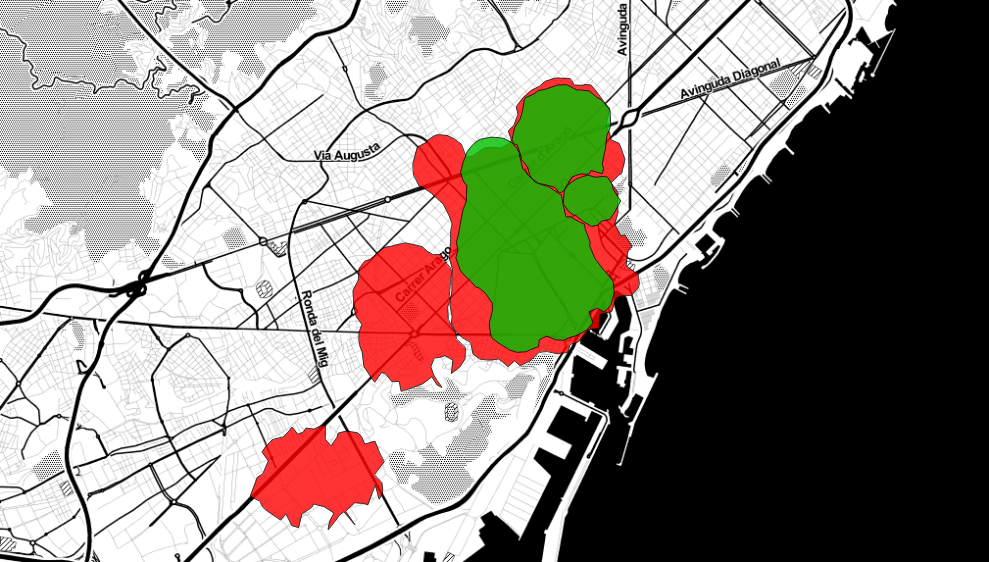
\includegraphics[scale=0.35]{mwc_nonmwc_1000_0125.png}
\end{figure}
\tiny{DBSCAN clusters of tweets during MWC vs a \textit{normal} day}
\end{frame}

\begin{frame}
\frametitle{Modelling Techniques}
Often Data Mining Techniques are combined together, or with traditional statistical methods, to yield better results:
\begin{itemize}
\item \textbf{Multivariate regression analysis + Bayesian Probabilistic Networks (BPN)} [cite];
\item Random Forest + Multivariate Adaptive Regression Splies (MARS) [cite];
\item Classification and Regression Trees (CART) [cite];
\item Genetic Mining Rule + Logit Model [cite];
\item \textbf{Frequent Item Sets [cite]};
\item Support Vector Machines (SVM); 
\item \textbf{Self Organizing Maps (SOM)};
%both present accuracies above 90%[cite]; SOM are only slighlty worst than SVM, which is unsuprising since they are trained in an unsuperviced fashion; they provide usefull graphic representations.
\end{itemize}
\end{frame}

\begin{frame}
\frametitle{Bayesian Approach}
In this case study[cite] it is used a mixed-model to predict the ocurrence of road accidents:
\begin{itemize}
\item<2-> Multivariate Poisson-lognormal regression analysis, which facilitates taking into account the covariance structure of the model response variables as well as
over-dispersion effects.
\item<3->  Bayesian Probabilistic Networks (BPN) that take into account aleatory and epistemic uncertainties as well as possibly non-linear dependencies between the risk indicating variables and the response variables.
\end{itemize}
The BPN is based on the regression model, but its parameters are updated by learning algorithms; the update \textit{only replaces the response variables that have been observed in conjunction with the accident}. This approach allows to cope with different degrees of completness of the dataset.\\
The methodology is illustrated using data of the Austrian rural motorway network (+/- 80 000 vehicles/day) and the quality of the prediction was found to be 73\%.
\end{frame}

\begin{frame}
\frametitle{Association Algorithm}
In this case study[cite] an association algorithm is used to obtain a descriptive analysis of accident high risk areas. This algorithm \textbf{identifies the accident circumstances that frequently occur together}. We are able to target the highest frequencies through a \textit{minimum support value}.\\
This algorithm was applied to road accident data in Belgian (1997-1999). 
%The dataset is long enough to limit random fluctuations in the accident counts and short enough to limit changes in road and traffic conditions.
Some factors that were frequently linked to accidents:
\begin{itemize}
\item "Left" turns;
\item Uneven views when approaching an intersection;
\item Rainy conditions;
\item Involvement of young pedestrians;
\end{itemize}
Some of these risk factors could be reduced with signing or roundabouts in these zones;
\end{frame}

\begin{frame}
\frametitle{What About Space?}
\begin{figure}
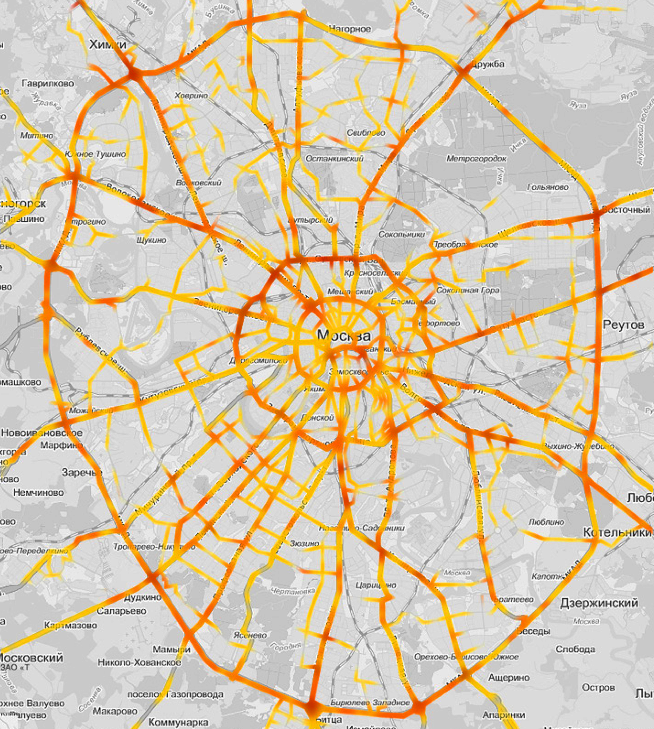
\includegraphics[scale=0.25]{accidentmap.png}
\caption{\tiny{Heat map of road accidents in Moscow; source: {\url http://mapsforhumans.com/2011/07/road-accidents-heat-map-of-moscow/}}}
\end{figure}
\end{frame}

\begin{frame}
\frametitle{What About Space? (cont.)}
Road accidents happen in time and \textbf{space}. The contact with the spatial dimension of the phenomena starts with the input dataset.\\
%Often accident data comes in very small units (e.g.: 100 m). Sometimes a spatial aggregation can be recommended, for getting rid of location error, and
%also to increase the magnitude of the results. We have to be very carefull on how-to do this generalisation.\\
The most frequent approach to represent the road structure is to use networks. Networks represent lanes as \textit{links} and intersections as \textit{nodes}.
\begin{figure}
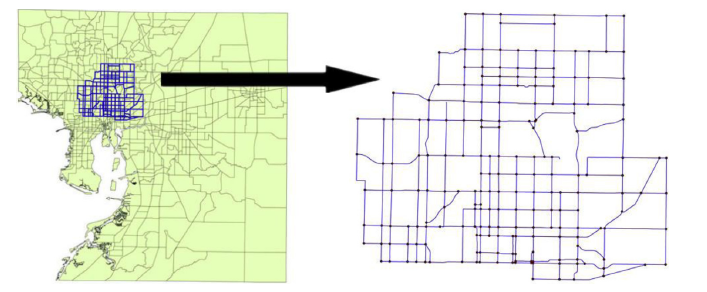
\includegraphics[scale=0.40]{road_network.png}
\caption{\tiny{Road network in  Hillsborough [cite]}}
\end{figure}
For longer roads, it may be actually useful to split them into \textbf{homogeneous sections}. %There are also \textit{gridifications} of these networks [cite].
\end{frame}

\begin{frame}
\frametitle{What About Space? (cont.)}
But the space dimension does not end up in the representation of the input variables (implicit). Space \textbf{relationships should also be explicitly stated in the model}.
\begin{itemize}
\item Spatial Auto correlation (as opposed to spatial independence) is an arrangement of the accidents where the locations are related to each other.
\item Numerous studies have shown that accounting for spatial correlation among the analyzed observations is a big step toward a better safety assessment [cite].
\item This is actually a \textit{weakness} of many models; on the Baysean Network model [cite], although acknowledged, spatial correlations were not considered in the development of the risk model; on conditionally autoregressive models (CAR) spatial effects are introduced as random.
\end{itemize}
Geographical Information Systems (GIS) can be a valuable tool for representing/integrating the different variables on a geographical space.
\end{frame}

\begin{frame}
\frametitle{Considering Space: A Simple Example}
Study of how circumstances affect people in episodes of bad weather [cite].Data from newspappers was collected for a period of 10 yrs, in the region of Calabria.
\begin{figure}
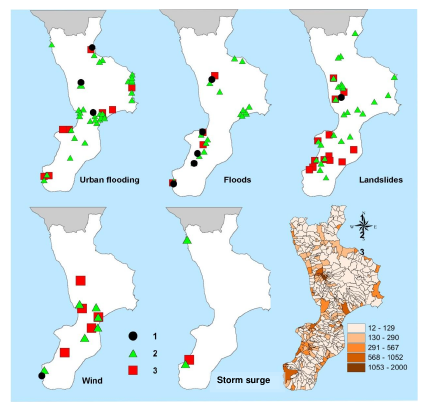
\includegraphics[scale=0.55]{damage_agent.png}
\caption{\tiny{Localisation of damage to people sorted according to the type of damaging agent. (1) Victims, (2) injured, and (3) involved people [cite]}}
\end{figure}
\end{frame}

\begin{frame}
\frametitle{Considering Space: A Simple Example (cont)}
\begin{columns}
  \begin{column}{0.5\textwidth}
    \begin{figure}
    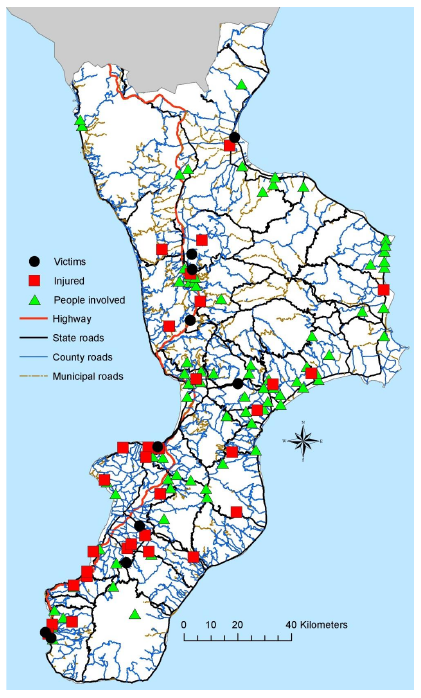
\includegraphics[scale=0.4]{damage2.png}
    \caption{\tiny{ Localisation of damage to people along the Calabria road network [cite]}}    
    \end{figure}
  \end{column}
  \begin{column}{0.5\textwidth}  
  \small{
  \begin{itemize}
  \item Urban flooding and flash floods were found to be the most damaging events;
  \item Drivers accounted for 84\% of the victims during these episodes.
  \item The mapping of damaging effects pointed out the regional sectors for which the high frequency of damaging events suggests planning further in-depth examinations; 
  \item The identification of these crictical points can support local regulator interventions, that might change damage incidences in the future.
  \end{itemize} }
  \end{column}
\end{columns}
\end{frame}

\begin{frame}
\frametitle{Considering Space: A more complex example}
Self Organizing Maps

\end{frame}

\begin{frame}
\frametitle{Targeting More Specific Aspects of Incidences:}
\begin{itemize}
\item Identify and describe secondary crashes;
\item Identify hots pots or "black zones", and model their behaviour;
\item Model crashes at specific type of road entity (e.g.: unsignalised intersections);
\item Classify incidences (e.g.: victims, injured, involved people);
\item Predict the type of accidents (casualties or damages);
\item ...
\end{itemize}
\end{frame}

\begin{frame}
\frametitle{Other Relevant Studies:}
\begin{itemize}
\item Predict traffic levels in unmeasured locations (Kriging)[cite];
\item Estimation of road traffic congestion (MCE, ANN)[cite];
\item Traffic simulation model (CA)[cite];
\item Traffic Forecast System[cite];
\item Predict travel time [cite];
\end{itemize}
\end{frame}

\begin{frame}
\frametitle{Visualization}
3D viz: give some "eye candy" examples
\end{frame}

\begin{frame}
\frametitle{References}
\end{frame}

\end{document}

%TODO: check how IESIM is written; test the times; if necessary remove animations; spread some slides; +4 (intervene: 2, one more for the hazard, one more for the intervene

